%%%%
%% poster.tex
%%
%% Copyright 2011 Jeffrey Finkelstein
%%
%% Except where otherwise noted, this work is made available under the terms of
%% the Creative Commons Attribution-ShareAlike 3.0 license,
%% http://creativecommons.org/licenses/by-sa/3.0/.
%%
%% You are free:
%%    * to Share — to copy, distribute and transmit the work
%%    * to Remix — to adapt the work
%% Under the following conditions:
%%    * Attribution — You must attribute the work in the manner specified by
%%    the author or licensor (but not in any way that suggests that they
%%    endorse you or your use of the work).
%%    * Share Alike — If you alter, transform, or build upon this work, you may
%%    distribute the resulting work only under the same, similar or a 
%%    compatible license.
%%    * For any reuse or distribution, you must make clear to others the 
%%    license terms of this work. The best way to do this is with a link to the
%%    web page http://creativecommons.org/licenses/by-sa/3.0/.
%%    * Any of the above conditions can be waived if you get permission from
%%    the copyright holder.
%%    * Nothing in this license impairs or restricts the author's moral rights.
%%%%
\documentclass{lposter}

\usepackage{amsmath}
\usepackage{amsthm}
\usepackage{complexity}
\usepackage{graphicx}
\usepackage{xcolor}
\usepackage{framed}
\usepackage{type1cm}

\title{Computational complexity of the linear matching templates (LMT) problem}
\author{Jeffrey Finkelstein}
\advisor{Steve Homer}
\department{Computer Science}
%\institute{Boston University}
\date{\today}
\year{2011}

\theoremstyle{definition} \newtheorem*{definition}{Definition}

\begin{document}
\begin{poster}

%% first column
\section{Motivation}

One of the goals of the study of syntax in natural languages is to explore how
the human mind understands sentential structure. For example, modern syntax
research suggests that the passive sentence

\begin{quote}
  \emph{The fries were eaten by John.}
\end{quote}

is less related to the corresponding active sentence

\begin{quote}
  \emph{John eats the fries}
\end{quote}

than to

\begin{quote}
  \emph{The children were happy in Paris.}
\end{quote}

Here, the past participle ``eaten'' yields the complex verb ``is eaten'' which
allows a ``by'' phrase. In this way, the passive sentence is more similar to a
sentence containing a predicate adjective.

We wish to determine how difficult it is for a computer to perform a matching
of word templates like the one in the above example.


\section{Problem definition}
Consider a linear tile with three cells. Each cell contains one color. Two
tiles can overlap wherever the cells have the same color. Given a set of tiles,
we wish to compute the linear layout of (possibly overlapping) tiles with the
shortest total length. Formally, the linear matching templates (LMT) problem
can be defined as follows:

\colorlet{shadecolor}{blue!40!gray!20}
\begin{shaded}
\begin{definition}\mbox{}

  Instance: a finite set of colors $\Sigma$, a finite set of sticks
  $T\subseteq\Sigma^3$, and $k\in\mathbb{N}$

  Question: Does there exist a layout $c\colon\{1,\ldots,k\}\to\Sigma$ such
  that for all tiles $(x, y, z)\in T$, there exists a position
  $n\in\{1,\ldots,k-2\}$ such that $c(n)=x$, $c(n+1)=y$ and $c(n+2)=z$?
\end{definition}
\end{shaded}


%% second column
\section{Linear programming characterization}
We can characterize these problems as integer linear programming problems so
that we may use the techniques and optimizations of general integer linear
programming solvers to decide these problems.

\colorlet{shadecolor}{blue!40!gray!20}
\begin{shaded}
\begin{definition}[Linear programming characterization]
  Let $C$ be a finite set of colors, let $k\in\mathbb{N}$ be the maximum
  length of the layout, let $n\in\mathbb{N}$ be the number of tiles, and let
  $s_{i,j}\in C$ be the symbol on tile $i$ at position $j$, where $1\leq i\leq
  n$ and $0\leq j\leq 2$. (We will assume for simplicity that $C$ is just the
  set $\{1, 2,\ldots, |C|\}$.)

  Let variable $x_{i,j}\in\{0, 1\}$, where $1\leq i\leq k$ and $1\leq j\leq
  |C|$, be defined by $x_{i, j} = 1$ if and only if symbol $j$ is at position
  $i$. Let variable $y_{i,j}\in\{0, 1\}$, where $1\leq i\leq k-2$ and $1\leq
  j\leq n$, be defined by $y_{i, j} = 1$ if and only if tile $j$ starts at
  position $i$.
    
  Let the constraints be as follows.
  \begin{itemize}
  \item[$\cdot$] Every tile must start at exactly one position:
    \begin{displaymath}
      \sum_{i = 1}^{k - 2}{y_{i, j}} = 1,\,\textnormal{for}\, 1\leq j\leq n
    \end{displaymath}
  \item[$\cdot$] Each position in the layout must have at most one symbol:
    \begin{displaymath}
      \sum_{j = 1}^{|C|}{x_{i, j}} = 1,\,\textnormal{for}\, 1\leq i\leq k
    \end{displaymath}
  \item[$\cdot$] The symbols of the layout must correspond to the symbols of
    the tiles:
    \begin{displaymath}
      y_{i, j} \leq x_{i + m, s_{j, m}}
    \end{displaymath}
    for $1\leq i\leq k - 2$, $1\leq j\leq n$, $0\leq m\leq 2$.
  \end{itemize}
    
  The linear matching templates problem is the problem of determining
  feasibility of the above linear programming instance.
\end{definition}
\end{shaded}


\section{\NP-complete variants}
The following variants of the LMT problem are \NP-complete.

{\bf LMT with intersecting sets}. If we allow each tile
to have a set of colors and allow tiles to overlap if the intersection of the
overlapping sets is non-empty, then the problem is \NP-complete.

\colorlet{shadecolor}{red!40!gray!20}
\begin{shaded}
\begin{proof}[Proof sketch]
  The reduction is from $\lang{HAMPATH}$. Transform each vertex of the graph
  into a tile, where the middle cell is the vertex, the left cell is the set of
  all incoming edges, and the right cell is the set of all outgoing edges. Then
  there is a layout of length $3|V| - (|V| - 1) = 2|V| + 1$ if and only if
  there is a Hamiltonian path in $G$.
\end{proof}
\end{shaded}

The original LMT problem is (basically) the restriction of this variant to sets
of tiles containing only singleton sets.

{\bf LMT chosen from bins}. If we are given a set of bins
containing tiles and require that one must be chosen from each bin, then the
problem is \NP-complete.

\begin{shaded}
\begin{proof}[Proof sketch]
  The reduction is again from $\lang{HAMPATH}$. For each vertex, create one bin
  and place in it one tile for each pair of incoming and outgoing edge, so that
  the left cell of the tile is one incoming edge, the middle cell is the
  vertex, and the right cell is one outgoing edge. Then there is a layout of
  length $2|V| + 1$ with one cell chosen from each bin if and only if there is
  a Hamiltonian path in $G$.
\end{proof}
\end{shaded}

The original LMT problem is (basically) the restriction of this variant to sets
of bins containing exactly one tile.

That the original problem is a restriction of these \NP-complete variants may
suggest that it is computationally \emph{easier}, though we can not currently
prove this.


\section{Example instance}
\begin{figure}
  \caption{An example instance of the LMT problem.}
  \includegraphics{example-instance}
\end{figure}

\begin{figure}
  \caption{A non-minimal layout of length 7.}
  \includegraphics{non-minimal}
\end{figure}

\begin{figure}
  \caption{A minimal layout of length 6.}
  \includegraphics{minimal}
\end{figure}


\section{Complexity}
The LMT problem is in \NP. So far we can neither prove that it is \NP-complete
nor that it is in \P.


\section{Further work}
\begin{itemize}
\item Determine if the linear matching templates problem is \NP-complete.
\item Determine the complexity of the following variants of the linear matching
  templates problem.
\item Consider the effect of probabilistically introduced wild-card tiles.
\end{itemize}


\end{poster}
\end{document}
